
	  
	  
	 


	  %%%%%%%%%%%%%%%%%%%%%%%%%%%%%%%%%%%%%%%%%%%%%%%%%%%%%%%%%%%%%%%%%%%%%%%%%%%%%%%%%%%%%%%%%%%%%
%%									   Chapitre 4	    								 %%
%%%%%%%%%%%%%%%%%%%%%%%%%%%%%%%%%%%%%%%%%%%%%%%%%%%%%%%%%%%%%%%%%%%%%%%%%%%%%%%%%%%%%%%%%%%%%
\chapter{ Réalisation et Déploiement  l'application}
\minitoc
\newpage
%%%%%%%%%%%%%%%%%%%%%%%%%%%%%%%%%%%%%
\section{Introduction}
Après avoir effectué  la modélisation, on peut désormais entamer la programmation et la réalisation du système. Dans cette partie, on abordera en premier lieu la description de notre \gls{sgbd} ainsi que les langages de programmation utilisés et par la suite on présentera les démarches de conception pour l'implémentation du système. 

\section{Les Systèmes de Gestion de Base de Données (SGBD)}
\subsection{Définition}
Les \gls{sgbd} sont des logiciels système destinés à stocker et à partager des informations dans une base de données, en garantissant la qualité, la pérennité et la confidentialité des informations, tout en cachant la complexité des opérations. En bref c'est un logiciel intermédiaires entre les utilisateurs et les bases de données. Une base de données est un magasin de données composé de plusieurs fichiers manipulés exclusivement par le \gls{sgbd}. Ce dernier cache la complexité de manipulation des structures de la base de données en mettant à disposition une vue synthétique du contenu.
\medskip

\subsection{Systèmes de Gestion de Base de Donne MYSQL}

\subsubsection{Pourquoi le choix de MYSQL?}

MYSQL est le SGBD qui est familiarisé par les informaticien du Polyclinique, le serveur qui y se trouve dispose déjà les ressource nécessaire pour démarrer  cette SGBD. Nous allons utilisé MYSQL car dans le cas contraire, les équipe qui va travailler au futur devra s'habituer à cette autre environnement, et cela va couté du temps.


\section{PHP avec le framwork Laravel}
\subsection{Pourquoi le choix de laravel?}
Laravel est le framwork les plus suggerére par le communauté du PHP aujourd'hui. Laravel est basé sur symfony mais on y introduit des différent amélioration.Laravel aussi rassemble des divers   avantage des  autre framwork et y intégré.
 laravel offre un avantage de taille, celui de separer la vue, le model et le Controller.l'avantage majeur est d'éviter le mélange de HTML avec du PHP. 

\medskip
 Il y a donc trois parties du cadre qui fonctionnent ensemble: les
modèles, les vues et les contrôleurs. Les contrôleurs sont la partie principale de la majeure partie
du travail. Ils se connectent aux modèles pour obtenir, créer ou mettre à jour des données et afficher les résultats sur les vues, qui contiennent la structure HTML   de l'application.

\subsection{Moteur de modèle de lame}
Laravel est livré avec un moteur de template appelé Blade. L'une des caractéristiques que le moteur de template Blade ne partage pas avec les
autres modèles populaires est sa permissivité; permettant l'utilisation de code PHP simple dans
les fichiers de moteur de template Blade.
Il est important de noter que les fichiers du moteur de .blade Blade ont .blade ajoutés aux noms
de fichiers juste avant l’habituel fichier .php qui n’est rien d’autre que l’extension du fichier. En tant que tel, .blade.php est l'extension de fichier résultante pour les fichiers de modèles Blade. Les
fichiers du moteur de modèle de lame sont stockés dans le répertoire resources /views.
\medskip

 
\subsection{Système de routage très facile à manœuvrer}
Vous pouvez définir les URL de votre application à l'aide d'itinéraires. Ces itinéraires peuvent
contenir des données variables, se connecter à des contrôleurs ou être intégrés dans des
middlewares. Middelware est un mécanisme de filtrage des requêtes HTTP. Ils peuvent être
utilisés pour interagir avec les requêtes avant qu'elles n'atteignent les contrôleurs et peuvent ainsi
modifier ou rejeter les demandes.

\subsection{  Eloquent ORM}
L'Eloquent est un ORM (Object Relational Model) inclus avec le Laravel. Il implémente le modèle d'enregistrement actif et est utilisé pour interagir avec des bases de données relationnelles.Pour connecter vos modèles à différents types de bases de données, Laravel propose son propre
ORM Eloquent avec un large éventail de fonctions avec lesquelles travailler.Le framework fournit également la migration et l'amorçage et propose également des restaurations.


\subsection{Artisan}
Artisan est l'outil en ligne de commande que vous pouvez utiliser pour contrôler certaines parties
de Laravel. Des nombreuses commandes sont disponibles pour créer des modèles, des contrôleurs et d'autres ressources nécessaires au développement.

\section{Création de squelete de projet laravel }
\subsection{Création du projet}
Nous devons avant tout installé Composer.
Ensuite pour installer Laravel, il suffit de taper la commande suivante dans votre bash :

\begin{verbatim}
composer create-project --prefer-dist laravel/laravel projectname
\end{verbatim}



\subsection{La structure des dossiers}
Après l'installation et la création de votre projet avec composer, nous allons voir la structure des dossiers et fichiers.
\
\begin{figure}[h]
	  	  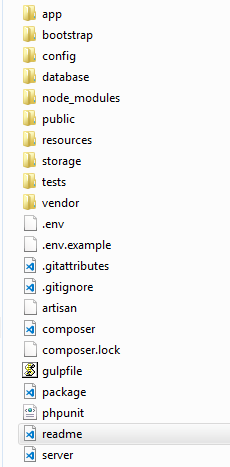
\includegraphics[scale=0.8]{Chapitre3/images/architecture}
	  
\end{figure}

Nous allons quasiment passer tout notre temps dans le dossier \emph{app},\emph{resources}, \emph{route}. Ce dossier contient presque tous les fichiers dont nous avons besoin pour coder notre application. Nous pouvons aussi installer des dépendances avec le gestionnaire de package de php : "Composer". Ces dépendances seront installées dans le dossier "vandor".











\section{Déploiement de l'application sur Apache}
Après avoir développé une application il faut pouvoir la déployer sur un serveur pour la rendre disponible par les utilisateurs On doit instaler l'environement suivant au préalable: Apache2,mysql, et PHP7.
\subsection{Configurer apache}
Rendez vous dans le dosier /etc/apache2
on cree un fichier nommé next.dev avec d'extention .conf dans le dossier site-availables
et on ejoute le code suivante: 

\begin{verbatim}
<VirtualHost *:80>
DocumentRoot /var/www/next.dev/public_html
<Directory "/var/www/next.dev/public_html">
Options +FollowSymLinks
AllowOverride all
Require all granted
</Directory>
<Directory "/var/www/next.dev/laravel">
Options +FollowSymLinks
AllowOverride all
Require all granted
</Directory>
ServerName next.dev
ServerAlias www.next.dev
ErrorLog /var/log/apache2/error.public.com.log
CustomLog /var/log/apache2/access.public.com.log combined
</VirtualHost>

\end{verbatim}

et puis executez le bach suivant:
\begin{verbatim}
a2ensite next.dev.conf
service apache2 reload
\end{verbatim}


rendez vous dans le dossier /etc et inserer dans le fichier nommé hosts la ligne suivante:
\begin{verbatim}
127.0.0.1       next.dev
\end{verbatim}

\subsection{Configurer l'application Laravel}
Par défaut, le dossier public du projet Laravel expose le contenu de l'application qui peut être
demandé de n'importe où par n'importe qui, le reste du code de l'application est invisible ou
inaccessible à quiconque sans les autorisations appropriées.

\medskip

Après avoir développé l'application sur votre machine de développement, celle-ci doit être
transmise à un serveur de production pour pouvoir y accéder

\begin{itemize}
	\item Étape 1
	Créez un dossier appelé laravel (ou tout ce que vous voulez) au même niveau que le dossier\begin{verbatim} public_html \end{verbatim}.
	
	Exemple :
	
	\begin{verbatim}
	
	/
	|--var
	|---www
	|----laravel
	|----public_html
	\end{verbatim}
	
	
	\item Étape 2
	Copiez tout sauf le dossier public de votre projet laravel (sur la machine de développement) dans
	le dossier laravel (sur l'hôte du serveur)
	
	\item Étape 3
	Ouvrez le dossier public de votre projet laravel (sur la machine de développement), copiez tout et
	collez-le dans le dossier \begin{verbatim} public_html (sur l'hôte du serveur)
	\end{verbatim}
	\item Étape 4
	Ouvrez maintenant le fichier index.php dans le dossier \begin{verbatim} public_html \end{verbatim}  sur l'hôte du serveur
	
	Changement:
	\begin{verbatim}
	require __DIR__.'/../bootstrap/autoload.php';
	\end{verbatim}
	À:
	\begin{verbatim}
	require __DIR__.'/../laravel/bootstrap/autoload.php';
	\end{verbatim}
	Et changer:
	\begin{verbatim}
	$app = require_once __DIR__.'/../bootstrap/app.php';
	\end{verbatim}
	À:
	\begin{verbatim}
	$app = require_once __DIR__.'/../laravel/bootstrap/app.php';
	Sauver et fermer.
	\end{verbatim}
	
	\item Étape 5
	Allez maintenant dans le dossier laravel (sur le laravel hébergement partagé) et ouvrez le fichier server.php
	Changement
	\begin{verbatim}
	require_once __DIR__.'/public/index.php';
	\end{verbatim}
	À:
	\begin{verbatim}
	require_once __DIR__.'../public_html/index.php';
	\end{verbatim}
	
	
	
	
	\item Étape 6
	
	Après avoir suivi toutes les étapes ci-dessus, créez un fichier .env dans le dossier laravel et
	ajoutez toute la variable d'environnement que vous avez utilisée du fichier .env du serveur local /
	de développement au fichier .env du serveur de production.
	
	
	\item Étape 7
	rendez vous sur l'url: http://next.dev/index.php
	
	
	
\end{itemize}




A la racine de notre application Laravel, on exécute la commande suivante : 
il faut copier le fichier laravel
\begin{verbatim}
php artisan key:generate
php artisan migrate
\end{verbatim}

Le déploiement effectué, notre application est maintenant accessible via l'URL : \\ \emph{"next.dev/index.php"}



\section{Présentation de l'application}
Nous allons faire une brève présentation de l'interface aussi bien que les fonctionnalités
de l'application. Notons au tout début que c’est une application utilisé en offline qui a
pour nomination : « NEXT app ». Cette application sera utilisé par l'administration et le secrétaire du polyclinique

\subsection{Fenêtre d'authentification}
\begin{figure}[h]
	\centering
	\includegraphics[width=0.55\linewidth]{"Chapitre4/images/authentification"}
	\caption{Fenêtre d'authentification}
	\label{Fenêtre d'authentification}
\end{figure}

Avant tout, l'utilisateur doit impérativement avoir un compte afin de logger sur l'application
\clearpage



\subsection{Le tableau de bord}

\begin{figure}[h]
	\centering
	\hspace*{-1.8cm}
	\includegraphics[width=1.2\linewidth]{"Chapitre4/images/dashboard"}
	\caption{Tableau de bord}
	\label{Tableau de bord}
\end{figure}

Après authentification, l’utilisateur sera redirigé directement au tableau de bord 

